\documentclass[12pt]{article}
 
\usepackage[margin=1in]{geometry}
\usepackage{amsmath,amsthm,amssymb, mathtools}
\usepackage[T1]{fontenc}
\usepackage{lmodern}
\usepackage{fixltx2e}
\usepackage[shortlabels]{enumitem}
\usepackage{mathrsfs}
\usepackage{kbordermatrix}


\usepackage{graphicx}
\usepackage{bbm}

\DeclarePairedDelimiter{\ceil}{\lceil}{\rceil}

\renewcommand{\kbldelim}{(}% Left delimiter
\renewcommand{\kbrdelim}{)}% Right delimiter
 
\newcommand{\N}{\mathbb{N}}
\newcommand{\R}{\mathbb{R}}
\newcommand{\Z}{\mathbb{Z}}
\newcommand{\Q}{\mathbb{Q}}
 
\newenvironment{theorem}[2][Theorem]{\begin{trivlist}
\item[\hskip \labelsep {\bfseries #1}\hskip \labelsep {\bfseries #2.}]}{\end{trivlist}}
\newenvironment{lemma}[2][Lemma]{\begin{trivlist}
\item[\hskip \labelsep {\bfseries #1}\hskip \labelsep {\bfseries #2.}]}{\end{trivlist}}
\newenvironment{exercise}[2][Exercise]{\begin{trivlist}
\item[\hskip \labelsep {\bfseries #1}\hskip \labelsep {\bfseries #2.}]}{\end{trivlist}}
\newenvironment{problem}[2][Problem]{\begin{trivlist}
\item[\hskip \labelsep {\bfseries #1}\hskip \labelsep {\bfseries #2.}]}{\end{trivlist}}
\newenvironment{question}[2][Question]{\begin{trivlist}
\item[\hskip \labelsep {\bfseries #1}\hskip \labelsep {\bfseries #2.}]}{\end{trivlist}}
\newenvironment{corollary}[2][Corollary]{\begin{trivlist}
\item[\hskip \labelsep {\bfseries #1}\hskip \labelsep {\bfseries #2.}]}{\end{trivlist}}
\newcommand{\textfrac}[2]{\dfrac{\text{#1}}{\text{#2}}}
\newcommand{\floor}[1]{\left\lfloor #1 \right\rfloor}

\newenvironment{amatrix}[1]{%
  \left(\begin{array}{@{}*{#1}{c}|c@{}}
}{%
  \end{array}\right)
}

\DeclareMathOperator*{\E}{\mathbb{E}}


\begin{document}

\title{Stochastic Processes II: Midterm}

\author{Chris Hayduk}
\date{March 25, 2021}

\maketitle

\begin{problem}{I}
\end{problem}

We have that,
\begin{align*}
E|N_n| &= E|\log(M_n) - \rho n|
\end{align*}

Note that $\rho n$ is a constant for any fixed $n$, and that $M_n$ is a finite sum of finite numbers for any fixed $n$. Thus,
\begin{align*}
E|N_n| < \infty
\end{align*}

for all $n \geq 0$. Moreover, since $H_n$ is predictable, $S_n = X_1 + \cdots X_n$, and $M_n$ is a product of these two, we have that $M_n$ can we determined from the values $X_n, \ldots X_0$ and $M_0$ as required. Lastly, we have,
\begin{align*}
M_{n+1} - M_n &= H_{k+1}X_{k+1}
\end{align*}

We have that $H_{k+1}X_{k+1} \leq 0$ when $X_{k+1} = -1$ and $H_{k+1}X_{k+1} \geq 0$ when $X_{k+1} = 1$.\\

Thus, we have,
\begin{align*}
N_{n+1} - N_{n} &= \log(M_{n+1}) - \rho (n+1) - (\log(M_{n}) - \rho n)\\
&= \log(M_{n+1}) - \rho n - \rho - \log(M_{n}) + \rho n\\
&= \log(M_{n+1}) - \rho - \log(M_{n})\\
&= \log(M_{n+1}) - (\log(M_{n}) + \rho)
\end{align*}

When $X_{k+1} = -1$, we have that $\log(M_n) + \rho > \log(M_{n+1})$ and so we get,



\begin{problem}{II}
\end{problem}

In order to inform our approach, let us first consider a random walk on the square $\{0, 1\}^2$ as a starting point. Then, with initial state $\vec{0} = (0, 0)$, we have the following drawing:

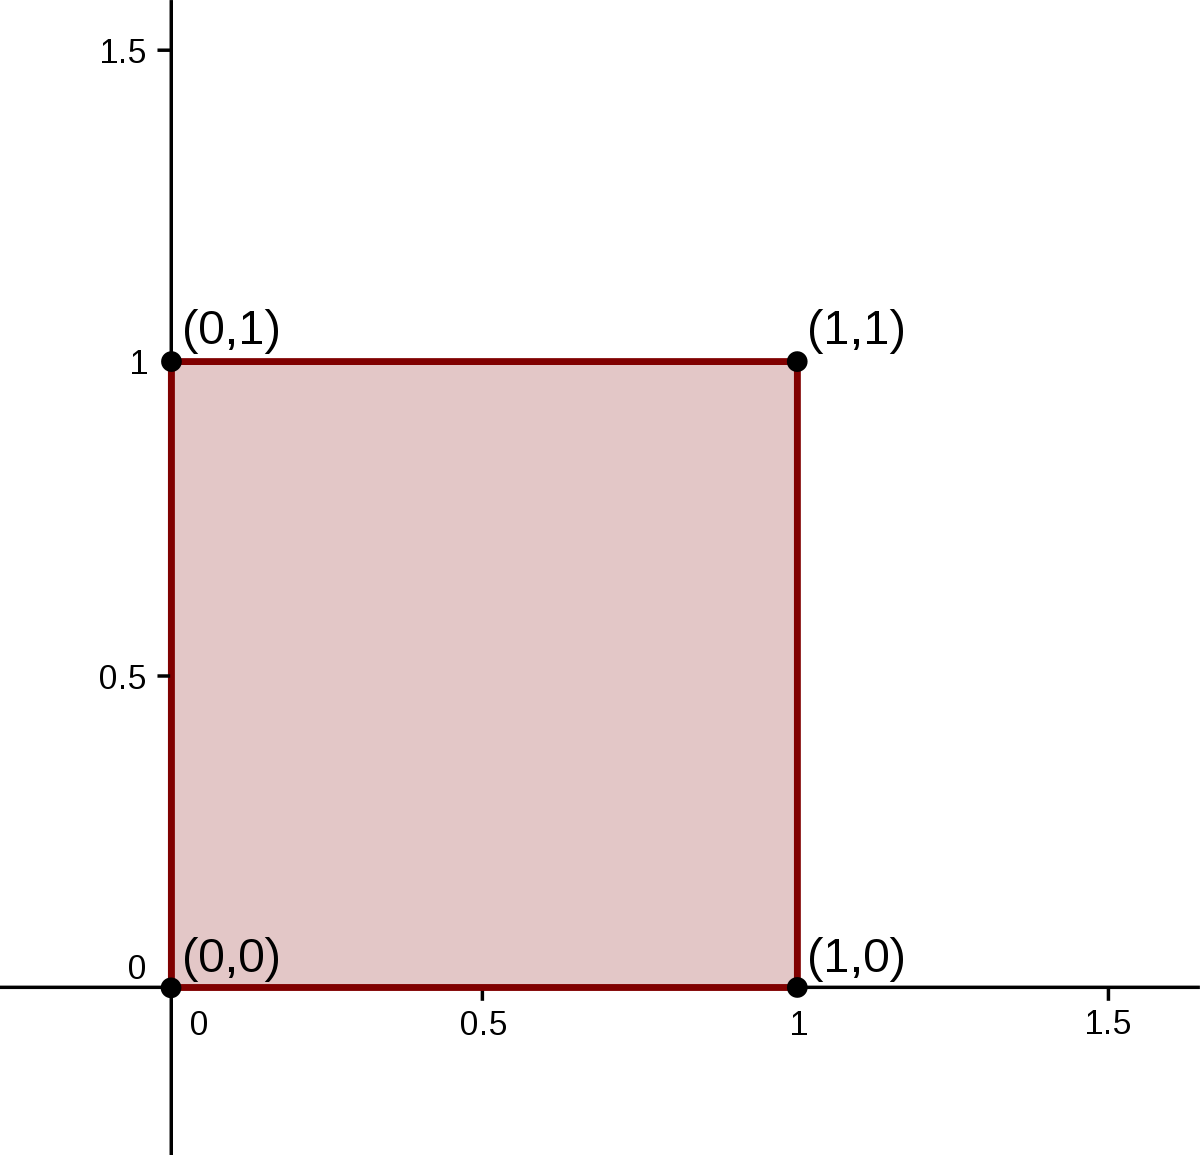
\includegraphics[scale=0.15]{unit_square}

We can set up the transition probability matrix fairly easily as follows,
\begin{align*}
p = \kbordermatrix{
    & (0,0) & (0,1) & (1,0) & (1,1) \\
    (0,0) & 0.5 & 0.25 & 0.25 & 0\\
    (0,1) & 0.25 & 0.5 & 0 & 0.25\\
    (1,0) & 0.25 & 0 & 0.5 & 0.25\\
    (1,1) & 0 & 0.25 & 0.25 & 0.5
  }
\end{align*}

Using numerical software to raise $p$ to the 10,000th power, we get,
\begin{align*}
p^{10000} &= \kbordermatrix{
    & (0,0) & (0,1) & (1,0) & (1,1) \\
    (0,0) & 0.25 & 0.25 & 0.25 & 0.25\\
    (0,1) & 0.25 & 0.25 & 0.25 & 0.25\\
    (1,0) & 0.25 & 0.25 & 0.25 & 0.25\\
    (1,1) & 0.25 & 0.25 & 0.25 & 0.25
  }
\end{align*}

Since all the entries of $p^{10000}$ are identical, we should have that $p$ raised to any other power will be the same matrix. Thus, in the case of lazy random walk on the square, we have $p^t(\vec{0}, \vec{x}) = 0.25$ for large $t$ and for all $\vec{x}$ in the state space. We will now attempt to generalize this to the hypercube.\\

From Section 2.3 in the text, we have that the stationary distribution on the hypercube is uniform on $\{0, 1\}^n$.  Now let us consider the transition matrix $p$ on the hypercube. Note that, since this is a lazy random walk, $p(x, x) > 0$ for all $x$ in the state space. Thus, every state has period $1$. That is, $p$ is aperiodic. Moreover, it is possible to reach any state $y$ from any state $x$ because the transition probability to any of $x$'s neighbors is positive and there must exist a path on the hypercube to any other vertex, otherwise the vertex would not be on the hypercube. Thus, $p$ is irreducible. Finally, we already have that $p$ has a stationary distribution, so that holds as well and we can apply Durrett Theroem 1.19 (Convergence Theorem), which states,
\begin{align*}
p^t(x,y) \to \pi(y)
\end{align*}

as $t \to \infty$. Hence, we have that $p^t(\vec{0}, x) \to \pi(x)$ for every state $x$ in the state space. But since the stationary distribution is uniform, this converges to the same value for every state $x$. Thus, for any choice of $x$ in the state space, we have that,
\begin{align*}
p^t(\vec{0}, x)
\end{align*}

is minimal for large $t$.

\begin{problem}{III}
\end{problem}

\begin{problem}{IV}
\end{problem}

\begin{enumerate}[label=(\Alph*)]

\item Suppose at time $t$, we have reached the point that all cards have been moved. Note that, by definition, the cards in the second deck are moved in the exact same order as the cards in the first deck are. Since every card has been picked by time $t$, every card in the second deck has been picked and moved in accordance with the first deck. Thus, we must have that $X_t = Y_t$ by this time $t$. Thus, we have that,
\begin{align*}
\tau_{\text{couple}} \leq \tau
\end{align*}

\item By Corollary 5.5 and our work above, we have that,
\begin{align*}
t_{\text{mix}} &\leq 4\max_{x,y} \E_{x,y} (\tau_{\text{couple}})\\
&\leq 4\max_{x,y} \E_{x,y} (\tau)
\end{align*}

Note that there is an equal probability of choosing any of the $n$ cards in the deck. That is, each cards is chosen with probability $1/n$. This is precisely the same as the coupon collector problem and so, by Proposition 2.3, we have,
\begin{align*}
E(\tau) = n \sum_{k=1}^n \frac{1}{k}
\end{align*}

Hence, we have that,
\begin{align*}
t_{\text{mix}} \leq 4n \sum_{k=1}^n \frac{1}{k}
\end{align*}

Note that $n \sum_{k=1}^n \frac{1}{k}$ is approximately $n\log(n)$ for large $n$. Hence, for large $n$ we have that,
\begin{align*}
t_{\text{mix}} &\leq \max_{x,y} 4n\log(n)\\
&= 4n\log(n)
\end{align*}
\end{enumerate}

\end{document}